\documentclass[11pt,utf8,notheorems,compress,t,aspectratio=169]{beamer}
\usepackage{etex}

\usepackage{pgfpages}
\usepackage[export]{adjustbox}

% Workaround for the issue described at
% https://tex.stackexchange.com/questions/164406/beamer-using-href-in-notes.
\newcommand{\fixedhref}[2]{\makebox[0pt][l]{\hspace*{\paperwidth}\href{#1}{#2}}\href{#1}{#2}}

\usepackage[english]{babel}

\usepackage[normalem]{ulem}
\usepackage{mathtools}
\usepackage{booktabs}
\usepackage{stmaryrd}
\usepackage{amssymb}
\usepackage{manfnt}
\usepackage{array}
\usepackage{ragged2e}
\usepackage{multicol}
\usepackage{tabto}
\usepackage{xstring}
\usepackage{proof}
\usepackage{agda}
\usepackage[all]{xy}
\xyoption{rotate}
\usepackage{tikz}
\usetikzlibrary{calc,shapes,shapes.callouts,shapes.arrows,patterns,fit,backgrounds,decorations.pathmorphing,positioning,svg.path}
\hypersetup{colorlinks=true}

\newcommand*\circled[1]{\tikz[baseline=(char.base)]{%
  \node[shape=circle,draw,inner sep=1pt] (char) {#1};}}

\DeclareFontFamily{U}{bbm}{}
\DeclareFontShape{U}{bbm}{m}{n}
   {  <5> <6> <7> <8> <9> <10> <12> gen * bbm
      <10.95> bbm10%
      <14.4>  bbm12%
      <17.28><20.74><24.88> bbm17}{}
\DeclareFontShape{U}{bbm}{m}{sl}
   {  <5> <6> <7> bbmsl8%
      <8> <9> <10> <12> gen * bbmsl
      <10.95> bbmsl10%
      <14.4> <17.28> <20.74> <24.88> bbmsl12}{}
\DeclareFontShape{U}{bbm}{bx}{n}
   {  <5> <6> <7> <8> <9> <10> <12> gen * bbmbx
      <10.95> bbmbx10%
      <14.4> <17.28> <20.74> <24.88> bbmbx12}{}
\DeclareFontShape{U}{bbm}{bx}{sl}
   {  <5> <6> <7> <8> <9> <10> <10.95> <12> <14.4> <17.28>%
      <20.74> <24.88> bbmbxsl10}{}
\DeclareFontShape{U}{bbm}{b}{n}
   {  <5> <6> <7> <8> <9> <10> <10.95> <12> <14.4> <17.28>%
      <20.74> <24.88> bbmb10}{}
\DeclareMathAlphabet{\mathbbm}{U}{bbm}{m}{n}
\SetMathAlphabet\mathbbm{bold}{U}{bbm}{bx}{n}

\usepackage{pifont}
\newcommand{\cmark}{\ding{51}}
\newcommand{\xmark}{\ding{55}}
\DeclareSymbolFont{extraup}{U}{zavm}{m}{n}
\DeclareMathSymbol{\varheart}{\mathalpha}{extraup}{86}

\graphicspath{{images/}}

\usepackage[protrusion=true,expansion=true]{microtype}

\setlength\parskip{\medskipamount}
\setlength\parindent{0pt}

\title{Towards multiversal modal operators for homotopy type theory}

\author{Ingo Blechschmidt}
\date{October 30th, 2023}

%\setbeameroption{show notes on second screen=bottom}
\newcommand{\jnote}[2]{\only<#1>{\note{\setlength\parskip{\medskipamount}\footnotesize\justifying#2\par}}}

%\useinnertheme[shadow=true]
\setbeamerfont{block title}{size={}}

\useinnertheme{rectangles}

\usecolortheme{orchid}
\usecolortheme{seahorse}
\definecolor{mypurple}{RGB}{253,73,34}
\definecolor{mypurpledark}{RGB}{100,0,150}
\setbeamercolor{structure}{fg=mypurple}
\setbeamercolor*{title}{bg=mypurple,fg=white}
\setbeamercolor*{titlelike}{bg=mypurple,fg=white}
\setbeamercolor{frame}{bg=black}

\usefonttheme{serif}
\usepackage[T1]{fontenc}
\usepackage{libertine}

% lifted from https://arxiv.org/abs/1506.08870
\DeclareFontFamily{U}{min}{}
\DeclareFontShape{U}{min}{m}{n}{<-> udmj30}{}
\newcommand\yon{\!\text{\usefont{U}{min}{m}{n}\symbol{'210}}\!}

\newcommand{\A}{\mathcal{A}}
\newcommand{\B}{\mathcal{B}}
\newcommand{\C}{\mathcal{C}}
\newcommand{\M}{\mathcal{M}}
\renewcommand{\AA}{\mathbb{A}}
\newcommand{\BB}{\mathbb{B}}
\newcommand{\pp}{\mathbbm{p}}
\newcommand{\MM}{\mathbb{M}}
\newcommand{\E}{\mathcal{E}}
\newcommand{\F}{\mathcal{F}}
\newcommand{\FF}{\mathbb{F}}
\newcommand{\G}{\mathcal{G}}
\newcommand{\J}{\mathcal{J}}
\newcommand{\GG}{\mathbb{G}}
\renewcommand{\O}{\mathcal{O}}
\newcommand{\K}{\mathcal{K}}
\newcommand{\NN}{\mathbb{N}}
\newcommand{\QQ}{\mathbb{Q}}
\newcommand{\RR}{\mathbb{R}}
\newcommand{\TT}{\mathbb{T}}
\newcommand{\PP}{\mathbb{P}}
\newcommand{\ZZ}{\mathbb{Z}}
\newcommand{\CC}{\mathbb{C}}
\renewcommand{\P}{\mathcal{P}}
\newcommand{\aaa}{\mathfrak{a}}
\newcommand{\bbb}{\mathfrak{b}}
\newcommand{\ccc}{\mathfrak{c}}
\newcommand{\ppp}{\mathfrak{p}}
\newcommand{\fff}{\mathfrak{f}}
\newcommand{\mmm}{\mathfrak{m}}
\newcommand{\defeq}{\vcentcolon=}
\newcommand{\defeqv}{\vcentcolon\equiv}
\newcommand{\Cov}{\mathrm{Cov}}
\renewcommand{\_}{\mathpunct{.}}
\newcommand{\?}{\,{:}\,}
\newcommand{\speak}[1]{\ulcorner\text{\textnormal{#1}}\urcorner}
\newcommand{\inv}{inv.\@}
\newcommand{\forces}{\vDash}

\setbeamertemplate{blocks}[rounded][shadow=false]

\newenvironment{indentblock}{%
  \list{}{\leftmargin\leftmargin}%
  \item\relax
}{%
  \endlist
}

% Adapted from https://latex.org/forum/viewtopic.php?t=2251 (Stefan Kottwitz)
\newenvironment<>{hilblock}{
  \begin{center}
    \begin{minipage}{9.05cm}
      \setlength{\textwidth}{9.05cm}
      \begin{actionenv}#1
        \def\insertblocktitle{}
        \par
        \usebeamertemplate{block begin}}{
        \par
        \usebeamertemplate{block end}
      \end{actionenv}
    \end{minipage}
  \end{center}}

\newenvironment{changemargin}[2]{%
  \begin{list}{}{%
    \setlength{\topsep}{0pt}%
    \setlength{\leftmargin}{#1}%
    \setlength{\rightmargin}{#2}%
    \setlength{\listparindent}{\parindent}%
    \setlength{\itemindent}{\parindent}%
    \setlength{\parsep}{\parskip}%
  }%
  \item[]}{\end{list}}

\tikzset{
  invisible/.style={opacity=0,text opacity=0},
  visible on/.style={alt={#1{}{invisible}}},
  alt/.code args={<#1>#2#3}{%
    \alt<#1>{\pgfkeysalso{#2}}{\pgfkeysalso{#3}}}
}

% https://tex.stackexchange.com/questions/172336/drawing-roman-laurel-leaves-spqr-in-tikz
\tikzset{
  laurel-wreath/.pic = {
    \fill svg{M14.4-24.6c-1.5-1.5-2.6-3.3-3.1-5.3l-.4-1.7c-.2-1.1-.2-4.1 .2-5.7 .2-.9 .3-1.3 .5-1.3l1.4 1.1 2.5 2.4c2.7 2.5 5.2 6 5.8 8 .2 .6-.5 .3-2.2-.9-1.6-1.3-3.3-2.6-5-3.8l.1 1.4c.2 1.4 .5 2.7 1.1 4.6s.8 2.5 .5 2.5l-1.4-1.3zm69.6 1.1 .3-1.2c.8-2.3 1.3-4.8 1.6-7.3l-1.5 1.1c-1.3 .9-2.6 1.9-3.7 3-1.6 1.1-2 1.3-2.1 1 .7-1.8 1.6-3.4 2.8-4.9 1.3-1.7 6.5-6.8 7-6.8 .2 0 .3 .2 .3 .5l.3 1.6c.3 2.2 .2 5.7-.5 7.4-.8 1.9-1.6 3.1-3 4.7-1.1 1.1-1.4 1.3-1.5 .9z};
    \fill svg{M10-29.4c-.8-1.1-1.4-2.2-2-4.1l-.7-3.5c-.2-3 .2-4.4 1.4-8.3l.5-1.4c.2-1.3 .3-1.9 .6-1.9 .3-.2 .6 .3 .7 .8s.9 2.2 1.9 3.6c1.4 2.2 2.7 4.4 3.9 6.6l.9 2.7c0 .6 0 .6-.3 .6-.6 0-4.9-4.4-5.8-6l-.2-.6-.1 1.7-.3 2.8c-.3 2.7-.3 3.8 0 5.5 .6 2 .5 2.4-.5 1.5zm79.2 .3 .4-2.4c.2-1.3 .2-2.7-.1-4.9l-.3-2.8v-1.6l-.7 1c-.8 1.3-5 5.5-5.5 5.5s-.5-.3 .2-1.9c.5-1.7 1.4-3.3 3.3-6.5 2.4-3.6 2.7-3.9 2.8-4.7 .5-1.3 .5-1.4 .8-1.2 .3 0 .6 .8 .6 1.5l.7 2.4c.9 2.7 1.1 3.6 1.2 6 .2 3.1-.5 6-2 8.2-.8 1.3-1.3 1.7-1.4 1.5z};
    \fill svg{M5-40c-.4-3.2-.1-6.5 .9-9.6 .5-1.1 1.6-2.8 2.2-3.4l1.3-1.6 2-2.7 .2 .6c.1 1.3 .4 2.6 .9 3.8l.3 1c.8 1.7 1.1 2.7 1.6 5.3 .6 2.5 .6 4.6 .2 4.6-.3 0-.9-.8-1-1.1l-.5-.8c-1.4-2-3-5.2-2.9-6.5-.9 2.7-2 5.4-3.5 7.9l-.3 .8-.3 .8c0 .5-.6 1.6-.8 1.6l-.3-.7zm89.2 .2-.2-.5-.3-.9-1.1-2.7-1.1-2.4c-.6-1.4-1.2-2.8-1.6-4.2l-.3 .9c-.3 1.3-1.6 3.9-3 6-1.3 2-1.6 2-1.5 0s1.1-6.3 2.2-9c.8-1.7 1.1-3.1 .9-4.1-.2-1.1 .5-.8 2.2 1.8 3.3 4.4 3.8 5.4 4.4 7.8 .6 2.4 .5 7.7-.3 7.8l-.3-.5z};
    \fill svg{M13.9-50.1c-.5-1.9-.8-3.9-.9-5.8-.2-1.6-.1-3.3 .1-4.9-.3 .8-1.7 2.5-4.2 5.1l-3 4.9-.3 .1c-.3 0-.3-2.2 0-3.3 .8-3 1.4-4.6 2.5-6.1 .9-1.3 1.7-1.9 2.5-2.5 1.1-.6 2.7-1.9 3.5-2.7 .9-.9 1.9-1.4 2.2-1.4v1.1l-.3 6.6c0 6.8 .2 6.3-1 8.9-.5 1.1-.8 1.1-1.1 0zm70.8-.4c-.8-2.2-.8-2.5-.7-6.3-.1-2.7-.1-5.5-.2-8.2-.3-1.6-.3-1.9 .5-1.6l.6 .5c1.4 1.4 3 2.5 3.9 3.1 1.3 .9 1.9 1.6 2.7 2.6l.6 .7 .2 .4 .2 .3c.8 .9 2 4.9 2 6.9 .2 1.9-.2 1.9-.9 .5-.7-1.4-1.5-2.7-2.6-4-1.6-1.5-3-3.2-4.2-5 .4 3 .3 6-.5 9 0 .8-.5 2.2-.8 2.3-.2 0-.5-.3-.8-1.2z};
    \fill svg{M16.4-58.5l.2-1.5 .3-3.7c.2-2.8 .3-3.5 1.1-5.4l.7-1.3-.5 .4-1 .7c-.5 .4-1.1 .8-1.5 1.3l-.5 .3-1.9 1.6c-2.2 1.6-2.7 2-3.9 3.6-.5 .8-1.1 1.3-1.3 1.3-.5 0 0-2.4 1.1-4.7 1.5-3.4 4.3-6 7.7-7.4l1.3-.4 1.9-.4 2-.5c1.4 0 1.4 0 1 1.1-.5 .8-.8 2-1.1 4.2-.3 2.3-1.1 4.5-2.2 6.5l-.4 .6c-.6 1.1-1.3 2.1-2 3.2-.5 .6-.8 .8-1 .5zm66.3-.2c-.8-.9-2.8-4.4-3.5-6.1-.6-1.3-.9-2.5-1.1-3.5-.2-2.1-.7-4.1-1.5-6 0-.3 0-.3 1.2-.3l2.1 .5 1.9 .4 1.2 .4 .6 .1 1 .6c3 1.4 5.7 4.6 6.8 8.5l.7 2.6c-.2 .6-.5 .5-1.4-.7-2.2-2.7-4.8-5-7.7-6.9l-1.7-1.3 .6 1.3c.3 .6 .6 1.2 .8 1.9l.3 2.5 .3 3.9c.3 2.4 .2 2.8-.6};
    \fill svg{M21.6-66.1l.4-1.1 .9-3.2c.3-1.9 1.1-3.3 2.4-4.7l.4-.8-1.2 .2-2.2 .3c-2.7 .3-5.3 1.2-7.7 2.5-.6 .5-1.3 .6-1.3 .3 0-.5 .9-1.9 2-2.9 .8-.9 2-1.9 3.2-2.6l.9-.4 2.2-1c.3-.2 1.3-.3 3.2-.1 3 0 4.1 .2 6.3 .7l1.1 .4c.5 .2 .6 .6 .3 .6-.5 0-1.4 .9-1.9 1.7l-1.2 1.8c-1.7 2.8-2.2 3.5-4.6 5.9l-3 2.7-.2-.3zm53.9-2c-2.7-2.8-3.5-3.8-5.4-6.8-.9-1.6-1.4-2.4-1.9-2.5l-.8-.5c-.3 0-.2-.5 .4-.6l1.1-.4c1.9-.6 3-.8 5.6-.9l3.3 .2c2 .6 3.8 1.5 5.4 2.8 .3 0 1.9 1.6 2.5 2.4l.9 1.8c0 .3-.3 .2-1.9-.6-2.8-1.4-4.4-1.9-7.7-2.2l-2.2-.5c-.9-.2-.9-.2-.6 .2 .6 .5 1.7 2 2.1 2.8l.9 2.5c.3 1.5 .6 3 .9 4.6l-2.6-2.3z};
    \fill svg{M34.1-78.7c-3.4-1.3-6.9-2.1-10.6-2.5-.9 0-1.4 0-2.3 .3-2 .5-2 0 0-1.3l2.8-1.2c1.4-.5 1.9-.5 3.8-.6 3.8-.2 6.1 .3 9.3 1.7l3.6 1.1 2.2 .3c1.3 0 1.7 0 2.7-.3 1.1-.3 2.8-1.1 2.8-1.3l-1.3-.9c-1.9-1.4-3.1-2.7-3.1-3.2l.8-.6c.9-.3 1.3-.2 2 .8 .5 .8 1.1 1.4 2.9 2.7 .2 .3 .3 .2 1.1-.3 .9-.8 2.4-2 2.6-2.7 .5-.6 .9-.8 1.8-.5l.8 .6c0 .5-1.4 1.7-3.2 3.2l-1.3 .9c0 .2 1.7 .9 2.9 1.3 .9 .3 1.4 .3 2.7 .3l2.2-.3c1.7-.4 3.4-1 5-1.7 2-.8 4.4-1.3 7.7-1.1 2 .2 2.5 .2 3.8 .6 .9 .3 2.2 .8 2.8 1.2 2 1.1 2 1.6 .2 1.3-1.6-.3-1.9-.3-4.4 0-2.4 .3-4.7 .8-7 1.6l-1.5 .6c-2.9 .3-5.9 .2-8.8-.3-1.7-.3-3.6-.9-6-2.1l-1.1-.4-1.3 .6c-4.5 2.2-9.6 3-14.6 2.2zm-6.3-9.1c};
  }
}

\newcommand{\pointthis}[3]{%
  \tikz[remember picture,baseline]{
    \node[anchor=base,inner sep=0,outer sep=0] (#2) {#2};
    \node[visible on=#1,overlay,rectangle callout,rounded corners,callout relative pointer={(0.3cm,0.5cm)},fill=blue!20] at ($(#2.north)+(-0.1cm,-1.1cm)$) {#3};
  }%
}

\tikzset{
  invisible/.style={opacity=0,text opacity=0},
  visible on/.style={alt={#1{}{invisible}}},
  alt/.code args={<#1>#2#3}{%
    \alt<#1>{\pgfkeysalso{#2}}{\pgfkeysalso{#3}}}
}

\newcommand{\hcancel}[5]{%
  \tikz[baseline=(tocancel.base)]{
    \node[inner sep=0pt,outer sep=0pt] (tocancel) {#1};
    \draw[red!80, line width=0.4mm] ($(tocancel.south west)+(#2,#3)$) -- ($(tocancel.north east)+(#4,#5)$);
  }%
}

\newcommand{\explain}[7]{%
  \tikz[remember picture,baseline]{
    \node[anchor=base,inner sep=2pt,outer sep=0,fill=#3,rounded corners] (label) {#1};
    \node[anchor=north,visible on=<#2>,overlay,rectangle callout,rounded corners,callout
    relative pointer={(0.0cm,0.5cm)+(0.0cm,#6)},fill=#3] at ($(label.south)+(0,-0.3cm)+(#4,#5)$) {#7};
  }%
}

\newcommand{\explainstub}[2]{%
  \tikz[remember picture,baseline]{
    \node[anchor=base,inner sep=2pt,outer sep=0,fill=#2,rounded corners] (label) {#1};
  }%
}

\newcommand{\squiggly}[1]{%
  \tikz[remember picture,baseline]{
    \node[anchor=base,inner sep=0,outer sep=0] (label) {#1};
    \draw[thick,color=red!80,decoration={snake,amplitude=0.5pt,segment
    length=3pt},decorate] ($(label.south west) + (0,-2pt)$) -- ($(label.south east) + (0,-2pt)$);
  }%
}

% Adapted from https://latex.org/forum/viewtopic.php?t=2251 (Stefan Kottwitz)
\newenvironment<>{varblock}[2]{\begin{varblockextra}{#1}{#2}{}}{\end{varblockextra}}
\newenvironment<>{varblockextra}[3]{
  \begin{center}
    \begin{minipage}{#1}
      \begin{actionenv}#4
        {\centering \hil{#2}\par}
	\def\insertblocktitle{}%\centering #2}
        \def\varblockextraend{#3}
	\usebeamertemplate{block begin}}{
        \par
        \usebeamertemplate{block end}
        \varblockextraend
      \end{actionenv}
    \end{minipage}
  \end{center}}

\setbeamertemplate{headline}{}

\setbeamertemplate{frametitle}{%
  \leavevmode%
  \vskip-1.6em%
  \begin{beamercolorbox}[dp=1ex,center,wd=\paperwidth,ht=2.25ex]{title}%
    \vskip0.5em%
    \bf\insertframetitle
  \end{beamercolorbox}%

  \vskip-0.77em\hspace*{-2em}%
  \textcolor{mypurpledark}{\rule[0em]{1.1\paperwidth}{2.4pt}}

  \vskip-0.4em%
}

\setbeamertemplate{navigation symbols}{}

\newcounter{framenumberpreappendix}
\newcommand{\backupstart}{
  \setcounter{framenumberpreappendix}{\value{framenumber}}
}
\newcommand{\backupend}{
  \addtocounter{framenumberpreappendix}{-\value{framenumber}}
  \addtocounter{framenumber}{\value{framenumberpreappendix}}
}

\newcommand{\insertframeextra}{}
\setbeamertemplate{footline}{%
  \begin{beamercolorbox}[wd=\paperwidth,ht=2.25ex,dp=1ex,right,rightskip=1mm,leftskip=1mm]{}%
    % \inserttitle
    \hfill
    \insertframenumber\insertframeextra\,/\,\inserttotalframenumber
  \end{beamercolorbox}%
  \vskip0pt%
}

\newcommand{\hil}[1]{{\usebeamercolor[fg]{item}{\textbf{#1}}}}
\newcommand{\hill}[1]{{\usebeamercolor[fg]{item}{#1}}}
\newcommand{\bad}[1]{\textcolor{red!90}{\textnormal{#1}}}
\newcommand{\good}[1]{\textcolor{mypurple}{\textnormal{#1}}}

\newcommand{\bignumber}[1]{%
  \renewcommand{\insertenumlabel}{#1}\scalebox{1.2}{\!\usebeamertemplate{enumerate item}\!}
}
\newcommand{\normalnumber}[1]{%
  {\renewcommand{\insertenumlabel}{#1}\!\usebeamertemplate{enumerate item}\!}
}
\newcommand{\bigheart}{
\includegraphics{heart}}

\newcommand{\subhead}[1]{{\centering\textcolor{gray}{\hrulefill}\quad\textnormal{#1}\quad\textcolor{gray}{\hrulefill}\par}}

\newcommand{\badbox}[1]{\colorbox{red!30}{#1}}
\newcommand{\infobox}[1]{\colorbox{yellow!70}{\color{black}#1}}

% taken from JDH "The modal logic of arithmetic potentialism and the universal algorithm"
\DeclareMathOperator{\possible}{\text{\tikz[scale=.6ex/1cm,baseline=-.6ex,rotate=45,line width=.1ex]{\draw (-1,-1) rectangle (1,1);}}}
\DeclareMathOperator{\necessary}{\text{\tikz[scale=.6ex/1cm,baseline=-.6ex,line width=.1ex]{\draw (-1,-1) rectangle (1,1);}}}
\DeclareMathOperator{\xpossible}{\text{\tikz[scale=.6ex/1cm,baseline=-.6ex,rotate=45,line width=.1ex]{\draw (-1,-1) rectangle (1,1); \draw[very thin] (-.6,-.6) rectangle (.6,.6);}}}
\DeclareMathOperator{\xnecessary}{\text{\tikz[scale=.6ex/1cm,baseline=-.6ex,line width=.1ex]{\draw (-1,-1) rectangle (1,1); \draw[very thin] (-.6,-.6) rectangle (.6,.6);}}}

% Taken from Todd Lehman (CC-BY-SA) at https://tex.stackexchange.com/a/44920/32372

\newcommand{\setisprime}[1]{
  % Sets \isprime based on #1.
  \ifnum#1=1 \gdef\isprime{0} \else \gdef\isprime{1} \fi
  \foreach \sip in {2, 3,5,...,#1} {
    \pgfmathparse{\sip*\sip>#1? 1:0}
    \ifthenelse{\pgfmathresult=1}{
      % Early-out if \sip^2 > #1.
      \breakforeach
    }{
      % Otherwise test if \sip divides #1.
      \pgfmathparse{Mod(#1,\sip)==0? 1:0}
      \ifthenelse{\pgfmathresult=1}{
        \gdef\isprime{0}
        \breakforeach
      }{}
    }
  }
}

\newcommand{\setxy}[1]{
  % Sets \x and \y to loction of cell #1.
  \pgfmathtruncatemacro{\x}{Mod(#1-1,\cols)}
  \pgfmathtruncatemacro{\y}{(#1-1) / \cols}
  \pgfmathtruncatemacro{\y}{\cols - 1 - \y}
  \pgfmathparse{2.5*(\x+.5)}\let\x\pgfmathresult
  \pgfmathparse{2.5*(\y+.5)}\let\y\pgfmathresult
}

\newcommand{\numlabel}[2]{
  % Draws label #2 at cell #1.
  \setxy{\n}
  \node[fill=none, text=black] at (\x,\y) {#2};
}

\newcommand{\drawpolygon}[2]{
  % Draws polygon with #2 vertexes at cell #1.
  \setxy{#1}
  \ifthenelse{#2>1}{ % Polygon must have at least 2 sides.
    \ifthenelse{#2<30}{ % Draw polygon if it has a small number of sides.
      \filldraw (\x,\y) +(90:1)
      \foreach \drawi in {1,...,#2} {-- +(\drawi/#2*360+90:1)} -- cycle;
    }{ % Else approximate with circle.
      \filldraw (\x,\y) circle(1);
    }
  }{}
}

\newcommand{\setpolygoncolor}[1]{
  % Sets color based on #1.
  \gdef\polycolor{black}
  \ifnum#1=2\gdef\polycolor{black!50!white}\fi
  \ifnum#1=3\gdef\polycolor{yellow!95!red}\fi
  \ifnum#1=5\gdef\polycolor{yellow!0!red}\fi
  \ifnum#1=7\gdef\polycolor{blue!75!green}\fi
  \ifnum#1=11\gdef\polycolor{blue!70!red}\fi
  \ifnum#1=13\gdef\polycolor{blue!40!red}\fi
  \ifnum#1=17\gdef\polycolor{green!50!blue}\fi
  \ifnum#1=19\gdef\polycolor{green!80!black}\fi
  \ifnum#1=23\gdef\polycolor{green!50!red}\fi
  \ifnum#1=29\gdef\polycolor{yellow!50!black}\fi
  \ifnum#1=31\gdef\polycolor{orange!50!black}\fi
  \ifnum#1=37\gdef\polycolor{red!50!black}\fi
  \ifnum#1=41\gdef\polycolor{purple!50!black}\fi
  \ifnum#1=43\gdef\polycolor{blue!50!black}\fi
  \ifnum#1=47\gdef\polycolor{green!50!black}\fi
  \ifnum#1=53\gdef\polycolor{white!50!black}\fi
  \ifnum#1=59\gdef\polycolor{white!50!black}\fi
  \ifnum#1=61\gdef\polycolor{white!50!black}\fi
  \ifnum#1=67\gdef\polycolor{white!50!black}\fi
}

\newcommand{\sieve}[2]{
  \def\cols{#1}
  \def\rows{#2}
  \begin{tikzpicture}[scale=.5]
  \pgfmathtruncatemacro{\nmax}{\rows * \cols}

  \foreach \n in {1,...,\nmax} {
    \begin{scope}[fill=gray, fill opacity=.05,
                  draw=gray, draw opacity=.10,
                  line width=4]
      \drawpolygon{\n}{\n}
    \end{scope}
    \setisprime{\n}
    \ifthenelse{\isprime=1}{
      \numlabel{\n}{\bf\n}
    }{
      \def\startintensity{.33}
      \def\incrintensity{.10}
      \def\intensity{\startintensity}

      \def\m{\n}
      \pgfmathtruncatemacro{\i}{\m / 2}

      % Divide \m by \i until \m is extinguished.
      % Increment \i each time it does not divide into \m.
      \whiledo{\m>1}{
        \setisprime{\i}
        \pgfmathparse{Mod(\m,\i)==0? 1:0}
        \ifthenelse{\pgfmathresult=1\and\isprime=1}{
          \setpolygoncolor{\i}
          \begin{scope}[fill=\polycolor, fill opacity=\intensity,
                        draw=\polycolor!85!black, draw opacity=\intensity,
                        line width=\intensity*1.5]
            \drawpolygon{\n}{\i}
          \end{scope}
          \pgfmathtruncatemacro{\m}{\m / \i}
          \pgfmathparse{\intensity + \incrintensity}\let\intensity\pgfmathresult
        }{
          \pgfmathtruncatemacro{\i}{\i - 1}
          \def\intensity{\startintensity}
        }
      }
      \begin{scope}[text=black, text opacity=.5]
        \numlabel{\n}{\scriptsize\n}
      \end{scope}
    }
  }

  \end{tikzpicture}
}


\newcommand{\triang}{\hil{$\blacktriangleright$}}
\newcommand{\concat}{\mathbin{{+}\mspace{-8mu}{+}}}

\newcommand{\astikznode}[2]{\tikz[baseline,remember picture]{\node[anchor=base,inner sep=0,outer sep=0.1em] (#1) {#2};}}
\newcommand{\astikznodecircled}[3]{\tikz[baseline,remember picture]{\node[anchor=base,circle,draw=#2,thick,inner sep=0,outer sep=0.05em] (#1) {#3};}}
\newcommand{\astikznodetransparentlycircled}[2]{\tikz[baseline,remember picture]{\node[anchor=base,circle,opacity=0,draw=white,text opacity=1,thick,inner sep=0,outer sep=0.05em] (#1) {#2};}}

\setbeamersize{text margin left=1.60em,text margin right=1.60em}

\newlength\stextwidth
\newcommand\makesamewidth[3][c]{%
  \settowidth{\stextwidth}{#2}%
  \makebox[\stextwidth][#1]{#3}%
}

\newcommand{\dnote}[1]{%
  \begin{tabular}{@{}m{2em}@{}m{0.80\textwidth}@{}}%
    \textdbend &#1%
  \end{tabular}%
  \par
}

\newcommand{\genalpha}{\mbox{$\hspace{0.12em}\shortmid\hspace{-0.62em}\alpha$}}

\usepackage{newunicodechar}

\newunicodechar{∇}{\ensuremath{\nabla}}
\newunicodechar{λ}{\ensuremath{\lambda}}
\newunicodechar{σ}{\ensuremath{\sigma}}
\newunicodechar{τ}{\ensuremath{\tau}}
\newunicodechar{∷}{\ensuremath{\!\!\!}}
\newunicodechar{⧺}{\ensuremath{\!\!\!}}
\newunicodechar{₁}{\ensuremath{_1}}
\newunicodechar{₂}{\ensuremath{_2}}
\newunicodechar{∈}{\ensuremath{\in}}

\begin{document}

\addtocounter{framenumber}{-1}

{\usebackgroundtemplate{\begin{minipage}{\paperwidth}\centering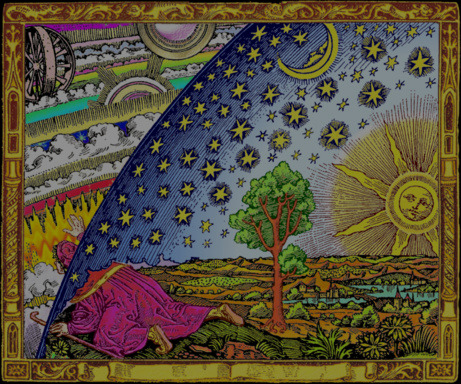
\includegraphics[height=\paperheight]{multiverse-faded}\end{minipage}}
\begin{frame}[c]
  \centering
  \color{white}

  \bigskip
  \bigskip
  \bigskip
  \bigskip

  \scriptsize
  \textit{-- an invitation --}

  \setbeamercolor{block body}{bg=black!100}
  \begin{minipage}{0.49\textwidth}
    \begin{block}{}
      \centering\normalsize\color{white}
      \hil{Towards multiversal modal operators for homotopy type theory}
    \end{block}
  \end{minipage}

  \bigskip
  \bigskip
  \bigskip
  \bigskip
  \bigskip
  \bigskip
  \bigskip
\end{frame}}

\definecolor{mypurple}{RGB}{150,0,255}
\setbeamercolor{structure}{fg=mypurple}

{\usebackgroundtemplate{\begin{minipage}{\paperwidth}
\includegraphics[height=\paperheight]{sea-of-clouds-2}\end{minipage}}
\begin{frame}{How should this notion be formalized in HoTT?}
  \jnote{5-}{
    The presented proof rests on the law of excluded middle and hence cannot
    immediately be interpreted as a program for finding suitable indices~$i < j$.
    However, constructive proofs are also possible (for instance by
    induction on the value of a given term of the sequence), and furthermore
    constructive proofs can be extracted from the presented classical proof.
  }

  \jnote{7-}{
    The class of well quasiorders is stable under cartesian products, lists and
    trees, by Dickson's Lemma, Higson's Lemma and Kruskal's Theorem,
    respectively. However, in their naive formulations, these are merely
    theorems of classical mathematics. For general constructive results, the
    definition of ``well'' needs to be improved.

    Classical texts often employ needless negations in their definitions; this
    is an XXX
  }

  \vspace*{-1em}
  \[ \astikznodetransparentlycircled{xm}{7}\!,
    \quad \astikznodetransparentlycircled{x0}{4}\!,
    \quad \only<1-2>{\astikznodetransparentlycircled{t1}{3}}\only<3->{\astikznodecircled{t1}{mypurple}{3}}\!,
    \quad \only<1>{\ldots}\pause \astikznodetransparentlycircled{x1}{1}\!,
    \quad \only<2>{\ldots}\pause \astikznodecircled{t2}{mypurple}{8}\!,
    \quad \only<3>{\ldots} \visible<4->{\astikznodetransparentlycircled{x2}{2}\!,}
    \quad \only<4->{\ldots} \]
  {\centering\begin{tikzpicture}[remember picture,overlay]
    \node[draw=mypurple, circle, thick, inner sep=0.1em] (t3) {\scriptsize$\leq$};
    \path[draw=mypurple,thick]
      (t1)
      to [out=-90, in=180] (t3)
      to [out=0, in=-90] (t2);
  \end{tikzpicture}\par}
  \medskip
  \pause

  \begin{block}{}
    \justifying
    \textbf{Thm.} Every sequence~$\alpha : \NN \to \NN$ is \hil{good} in that
    there exist~$i < j$ with~$\alpha\,i \leq \alpha\,j$.
  \end{block}
  \pause
  \vspace*{-0.6em}
  \emph{Proof.} \emph{(offensive?)} By~\badbox{\textsc{lem}}, there is a
  minimum~$\alpha\,i$.
  Set~$j \defeq i + 1$. \qed\par
  \pause

  \textbf{Def.} (classically) A quasiorder~$X$ is \hil{well} iff every sequence~$\NN \to X$ is good.

  \textbf{Examples.} (classically)\ $(\NN,{\leq}),\ \ X \times Y,\ \ X^*,\ \ \mathrm{Tree}(X).$
  \bigskip
  \pause

  \emph{A naive formalization attempt:}

  \textbf{Def.} $\displaystyle\mathsf{Well}_\infty(X,{\leq}) \defeq
    \prod\limits_{\alpha \? \NN \to X} \, \Bigl\|\sum\limits_{i \? \NN} \sum\limits_{j \? \NN}
      i < j \times \alpha\,i \leq \alpha\,j\Bigr\|_{-1}$
  \pause
  \qquad\scalebox{1.5}{\dbend}
  \medskip

  \begin{itemize}
    \item[\bad{\xmark}] philosophically~strenuous  %: needless reference of the transfinite
    \item[\bad{\xmark}] not practical  %: cannot verify closure properties
    \item[\bad{\xmark}] not faithful(?)  %: missing out on some sequences
  \end{itemize}
\end{frame}}

\begin{frame}{Sequences provided by \textsc{lem}}
  \justifying
  \begin{block}{}
    \justifying
    \textbf{Lemma.} Let~$X$ be a well quasiorder. Let~$\alpha : \NN \to X$ be a
    sequence. Assuming~\bad{\textsc{lem}}, there merely is a monotonic
    subsequence~$\alpha\,i_0 \leq \alpha\,i_1 \leq \cdots$.
  \end{block}
  \vspace*{-0.6em}
  \emph{Proof.} The set
  \[ I \defeq \{ i \in \NN \,|\, \neg\mathop{\exists}\limits_{j \in \NN} i < j \times \alpha\,i \leq \alpha\,j
  \} \]
  cannot be in bijection with~$\NN$, as else the~$I$-extracted subsequence
  of~$\alpha$ would not be good. By~\bad{\textsc{lem}}, the set~$I$ is finite.
  Any index~$i_0$ larger than all the indices in~$I$ is a suitable starting
  point for a monotonic subsequence. \qed
  \medskip
  \pause

  \begin{block}{}
    \justifying
    \textbf{Prop.} Let~$X$ and~$Y$ be well quasiorders.
    Assuming~\bad{\textsc{lem}},~$X \times Y$ is well.
  \end{block}
  \vspace*{-0.6em}
  \emph{Proof.} Let an infinite sequence~$\gamma : \NN \to X \times Y$ be
  given. Write~$\gamma\,k = (\alpha\,k,\beta\,k)$. By the lemma, there is a
  monotonic subsequence~$\alpha\,i_0 \leq \alpha\,i_1 \leq \cdots$. Because~$Y$
  is well, there are indices~$n < m$ such that~$\beta\,i_n \leq \beta\,i_m$. As
  also~$\alpha\,i_n \leq \alpha\,i_m$, the sequence~$\gamma$ is good.
  \medskip
  \pause

  \dnote{\emph{We cannot trust~\bad{\textsc{lem}}-provided sequences to be
  available in the type~$\NN \to \NN$. Similarly with~\bad{\textsc{dc}}.}}
\end{frame}

\begin{frame}{Sequences depending on an environment}
  Let~$X$ be an hset such that there is no surjection~$\NN \twoheadrightarrow X$.
  Then the type~$\NN \to X$ misses the \hil{generic enumeration}~$\genalpha$ of~$X$.
  \medskip
  \pause

  \emph{Idea:} Approximate (fictitious) surjections~$\NN \twoheadrightarrow X$
  by finite sequences~$\sigma = x_0 \ldots x_{n-1} \? X^*$. \\ Over time, such an
  approximation can grow to
  \begin{enumerate}
    \item one of $\sigma y$, where~$y \? X$, so it becomes \emph{more defined}; or
    \item one of~$\sigma \tau$, where~$\tau \? X^*$ such that~$a \in
    \sigma\tau$, so it becomes \emph{more surjective}.
  \end{enumerate}
  \medskip
  \pause

  For~$k : \NN$ and~$a : X$, the expression~``$\genalpha\,k = a$'' does not
  denote a proposition but rather a \hil{stage-dependent proposition}~$X^* \to
  \mathsf{Prop}$, namely $\lambda x_0 \ldots x_{n-1}.\ k < n \times x_k = a$.
  \medskip
  \pause

  Given a stage-dependent proposition~$P$, $\hil{$\nabla P$}\,\sigma$ expresses that no
  matter how~$\sigma$ evolves to a better approximation~$\tau$,
  eventually~$P\,\tau$ will hold:
  \AgdaHide{
  \begin{code}
    {-# OPTIONS --no-prop --no-import-sorts --allow-unsolved-metas #-}
    open import Agda.Primitive using (Set)
    Prop = Set
    postulate
      X : Set
      X* : Set
      [] : X*
      _∷_ : X* → X → X*
      _⧺_ : X* → X* → X*
      _∈_ : X → X* → Prop
    module Foo where
  \end{code}
  }
  {\small\begin{code}
      data ∇ (P : X* → Prop) (σ : X*) : Prop where
        now : P σ → ∇ P σ
        later₁ : ((y : X) → ∇ P (σ ∷ y)) → ∇ P σ
        later₂ : (a : X) → ((τ : X*) → a ∈ (σ ⧺ τ) → ∇ P (σ ⧺ τ)) → ∇ P σ
  \end{code}}

  \vspace*{-0.8em}
  For instance, for~$P\,x_0 \ldots x_{n-1} \defeq \exists_{k : \NN} (k < n
  \times x_k = a)$, we have~$\nabla P \, \varepsilon$. \quad ``$\genalpha$ is surjective''
\end{frame}

\begin{frame}{Well quasiorders revisited}
  \emph{A naive formalization attempt:}

  \textbf{Def.} $\displaystyle\mathsf{Well}_\infty(X,{\leq}) \defeq
    \prod\limits_{\alpha \? \NN \to X} \, \Bigl\|\sum\limits_{i \? \NN} \sum\limits_{j \? \NN}
      i < j \times \alpha\,i \leq \alpha\,j\Bigr\|_{-1}$
  \pause
  \qquad\scalebox{1.0}{\dbend}
  \bigskip 

  \emph{An inductive rephrasing:}

  \textbf{Def.} $\displaystyle\mathsf{Well}(X,{\leq}) \defeq
    \nabla \mathsf{Good} \, \varepsilon$, where~$\mathsf{Good}\,x_0 \ldots
    x_{n-1} \defeq \mathop{\exists}\limits_{i:\NN}\mathop{\exists}\limits_{j:\NN} (i < j \times x_i \leq
    x_j)$ and
  {\vspace*{-0.7em}\small\begin{code}
    data ∇ (P : X* → Prop) (σ : X*) : Prop where
      now : P σ → ∇ P σ
      later : ((y : X) → ∇ P (σ ∷ y)) → ∇ P σ
  \end{code}}

  \vspace*{-0.8em}
  In other words: \emph{A quasiorder~$X$ is well iff the generic sequence~$\NN \to X$
  is good.}

  \begin{block}{}
    \justifying
    \textbf{Prop.} Let~$X$ and~$Y$ be well quasiorders.
    \good{Without} assuming~\bad{\textsc{lem}},~$X \times Y$ is well.
  \end{block}

  \dnote{We have~$\mathsf{Well}(X,{\leq}) \to
  \mathsf{Well}_\infty(X,{\leq})$, but the converse only holds in presence of \hil{bar
  induction}. \emph{How much stronger exactly is the inductive rephrasing?}}
\end{frame}

{\usebackgroundtemplate{\begin{minipage}{\paperwidth}\vspace*{4.95cm}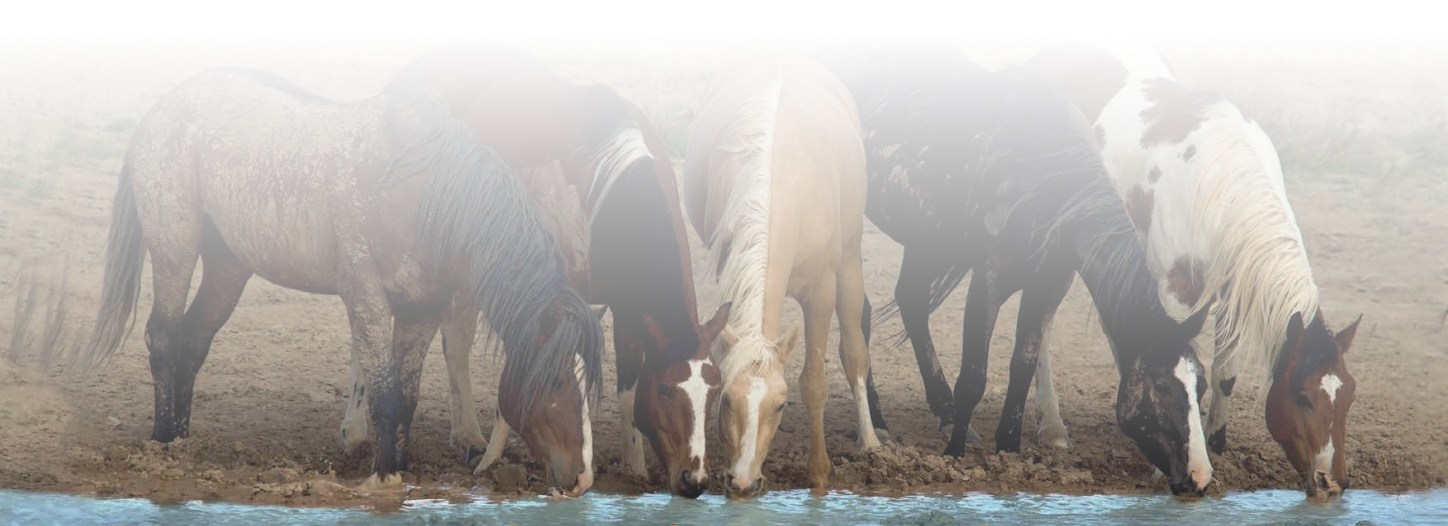
\includegraphics[width=\paperwidth]{topos-horses}\end{minipage}}
\begin{frame}{Slide about toposes}
  (something about overloading of the logical connectives)
\end{frame}}

{\usebackgroundtemplate{\begin{minipage}{\paperwidth}\vspace*{5.95cm}
\includegraphics[width=\paperwidth]{fr1}\end{minipage}}
\begin{frame}{Maximal ideals as convenient fictions}
  \jnote{1}{
    The theorem on the slide is a generalization of a fact from undergraduate
    linear algebra: Over a field, no surjective matrix can have more rows than
    columns. (``Surjective'' here means that the induced linear map is
    surjective.)
  }

  \jnote{6-7}{
    The slide presents a standard proof as offered by most textbooks on
    commutative algebra. The proof is quite efficient from a viewpoint of
    mathematical organization, as it quickly succeeds in reducing to the field
    situation. As such, it is short and memorable.

    However, the proof can also be critized for appealing to the transfinite
    two times; the methods of the proof are at odds with the concreteness of
    the statement of the theorem---from given equations witnessing
    surjectivity,~$Mv_i = e_i$, we are asked to deduce the equation~$1 = 0$.

    For this reason, the theorem and its classical proof are often used as case
    studies for tools and techniques aiming to extract constructive content
    from classical proofs. One such technique employs constructive forcing.
    The first(?)\@ constructive proof, found directly without using extraction
    techniques, is laid out in a
    \fixedhref{https://www.ams.org/journals/proc/1988-103-04/S0002-9939-1988-0954974-5/S0002-9939-1988-0954974-5.pdf}{beautiful short note by Richman}.
  }

  \jnote{8-9}{
    For the countable case, there is an iterative construction of a maximal
    ideal, making do without any decidability assumptions (due to Krivine,
    later later clarified by Berardi and Valentini). It is a parlor trick,
    resulting in a subset which formally verifies the axioms for a maximal
    ideal but without carrying out any actual work. Indeed, the resulting ideal
    will in general not be a detachable subset of the ring.

    Surprisingly, there is still computational content in this construction, as
    explored in \fixedhref{https://arxiv.org/abs/2207.03873}{this joint paper
    with Peter Schuster}; one interpretation of our observation is that classical
    proofs don't ``really'' require a maximal ideal; they just use that notion
    for structuring hidden computations.
  }

  \jnote{9}{
    In a suitable topos, the ring appears countable. Hence we can
    carry out the iterative maximal ideal construction there. The resulting ideal
    will not be part of the base universe (instead, from the point of view of
    the base universe we will just have constructed a certain sheaf of ideals on a
    certain pointfree space), but bounded first-order consequences of its
    existence still pass down to the base.
  }

  \jnote{10}{
    Unwinding all the definitions from toposes and from the
    iterative maximal ideal construction, and eliminating the application
    of~\textsc{lem} from the classical proof presented before, we mechanically
    arrive at the constructive direct proof presented on the slide.
  }

  \begin{block}{}
    \textbf{Thm.}
    Let~$M$ be a surjective matrix with more rows than columns over a
    commutative ring~$A$. Then~$1 = 0$ in~$A$.
  \end{block}

  \only<1-9>{
    \visible<2->{\emph{Proof.} (classical) \bad{Assume not.}}
    \visible<3->{Then there is~a \bad{maximal ideal} $\mmm$.}
    \visible<5->{The matrix is surjective over~$A/\mmm$.}
    \visible<6->{Since~$A/\mmm$ is a field, this is a contradiction to basic linear algebra.\qed}
  }

  \only<4-9>{\medskip\par\centering\scalebox{0.9}{\centering\begin{tikzpicture}
    \node (0) at (0,1) {$(0) = \{0\}$};
    \node (1) at (0,5) {$(1) = \ZZ$};
    \node (2) at (-2,4) {$(2)$};
    \node [right of=2] (3) {$(3)$};
    \node [below of=2] (4) {$(4)$};
    \node [below of=2, xshift=0.7cm] (6) {$(6)$};
    \node [right of=3] (5) {$(5)$};
    \node [right of=5] (7) {$(7)$};
    \node [right of=7] (7d) {$\ldots$\phantom{(}};
    \node [right of=7d, xshift=3cm, yshift=-2cm] (max)
    {\vbox{\small{\it maximal among the proper ideals} \\ \medskip \hspace*{-6.75em}\textbullet \quad $\neg(1 \in
    \mmm)$ \\ \medskip \textbullet \quad $\neg\bigl(1 \in \mmm + (x)\bigr) \Rightarrow x \in \mmm$}};
    \node [below of=4] (8) {$(8)$};
    \node [right of=8, xshift=3cm] (8d) {$\ldots$};
    \draw (0) -- (8);
    \draw (0) -- (8d);
    \draw (0) -- (6);
    \draw (2) -- (1);
    \draw (3) -- (1);
    \draw (5) -- (1);
    \draw (7) -- (1);
    \draw (7d) -- (1);
    \draw (4) -- (2);
    \draw (8) -- (4);
    \draw (6) -- (2);
    \draw (6) -- (3);
    \draw [mypurple!30, thick, shorten <=-2pt, shorten >=-2pt, ->] (max) to [out=120, in=-30] (7d);
    \begin{pgfonlayer}{background}
      \draw[decorate, very thick, draw=mypurple!30]
        ($(2.south west) + (8pt, 0)$) arc(270:180:8pt) --
        ($(2.north west) + (0, -8pt)$) arc(180:90:8pt) --
        ($(7d.north east) + (-8pt, 0)$) arc(90:0:8pt) --
        ($(7d.south east) + (0, 8pt)$) arc(0:-90:8pt) --
        cycle;
    \end{pgfonlayer}
  \end{tikzpicture}\par}\par}

  \pause
  \pause
  \pause
  \pause
  \pause
  \pause
  \raggedright

  \only<7-9>{
    \emph{Does there exist a maximal ideal?}
    \pause
    \good{Yes}, if~$A$ is countable.
    In the general case: \bad{No}\pause, but \good{yes} in a \emph{suitable topos}, and
    \emph{bounded first-order consequences} of its existence there \good{do hold} in
    the base.
    \pause
  }

  \only<10>{
    \emph{Proof.} (constructive, special case) Write~$M =
    \left(\begin{smallmatrix}x\\y\end{smallmatrix}\right)$. By surjectivity,
    we have~$u, v \? A$ with
    \[
      u \left(\begin{smallmatrix}x\\y\end{smallmatrix}\right) = \left(\begin{smallmatrix}1\\0\end{smallmatrix}\right)
      \quad\text{and}\quad
      v \left(\begin{smallmatrix}x\\y\end{smallmatrix}\right) = \left(\begin{smallmatrix}0\\1\end{smallmatrix}\right).
    \]
    Hence
    $
      1 = (vy) (ux) = (uy) (vx) = 0
    $. \qed
  }
\end{frame}}

\newcommand\ytl[2]{%
  \parbox[b]{4.5em}{\hfill{#1}~$\cdots\cdots$~}%
  \makebox[0pt][c]{\color{mypurple}$\bullet$}{\color{mypurple}\vrule}\quad%
  \parbox[c]{9.3cm}{\vspace{7pt}\raggedright#2\\[7pt]}%
  \\[-2.0pt]}
\begin{frame}{A brief timeline}
  \jnote{4}{
    Gödel's proof is by the \hil{$L$-translation}, where $L$ is the
    ``constructible universe''. This translation ``relativizes quantification
    to~$L$'', for instance the~$L$-translation of
    \[ \varphi \defeqv \bigl(\forall x\_ \exists y\_ \ldots\bigr) \qquad\text{is}\qquad
    \varphi^L \equiv \bigl(\forall(x \in L)\_ \exists(y \in L)\_ (\ldots)^L\bigr). \]
    We can then verify, in a weak metatheory such as~\textsc{pra}, that for
    every formula~$\varphi$ in the language of set theory:
    If $\textsc{zfc}\text{+}\textsc{ch} \vdash \varphi$, then $\textsc{zf} \vdash
    \varphi^L$.

    Specializing to~$\varphi \defeqv \bot$ we obtain in particular: If~\textsc{zfc} is
    inconsistent, then so is~\textsc{zf}. The axiom of choice does not
    introduce new inconsistencies.

    In modern semantic language: While the axiom of choice and~\textsc{ch} might fail in the
    base universe~$V$ (= the class of all sets), they always hold in~$L$.
    Gödel's~$L$ was the first \emph{inner model} (= class-sized model of set
    theory) explicitly studied, nowadays we know many.
  }

  \jnote{5}{
    For his proof, Cohen invented the technique of \emph{forcing}, situated in
    classical mathematics where the base universe~$V$ is assumed to validate
    the axioms of~\textsc{zfc}.

    Recall that a given ring~$R$ or group can be extended in various ways, to include
    ``generic elements'' as in~$R[X]$ or elements with prescribed relations as
    in~$R[X]/(X^2+1) =\vcentcolon R[i]$. The idea of forcing is to construct
    similar such extensions, but not of rings but of universes (traditionally set-sized models
    of~\textsc{zf} or~\textsc{zfc}, but also class-sized models, or models
    of intuitionistic set theories, or models of type theories, or even models
    of arithmetic).

    In semantic language, from a high level the idea of Cohen's independency proof is the following: Whether
    the base universe~$V$ contains a cardinal number intermediate
    between~$\aleph_0$ and~$2^{\aleph_0}$ is uncertain. But there is a certain
    extension of the base universe---constructed by forcing---which does
    contain such a number. Like the base~$V$, this forcing extension still
    validates the axioms of~\textsc{zfc}. Hence there cannot be a
    \textsc{zfc}-proof of~\textsc{ch}, as in Cohen's extension~$\neg\textsc{ch}$
    holds.

    Syntactically, Cohen's forcing provides us with an explicit formula
    translation~$\varphi \mapsto \varphi^C$ such that~\textsc{pra} proves:
    For every formula~$\varphi$, if~$\textsc{zfc}{\text{+}}\neg\textsc{ch} \vdash \varphi$,
    then~$\textsc{zfc} \vdash \varphi^C$.
    \bigskip
  }

  \jnote{6}{
    Joel David Hamkins argues: In view of our rich experience with worlds which
    validate~\textsc{ch} and worlds which don't, we shouldn't be surprised that
    no proposed new axiom for settling~\textsc{ch} is ultimately convincing.

    Instead, we should embrace the multiverse of all models of set theory and
    explore how the truth values of statements of interest change when we
    travel the multiverse (for instance, by passing from a universe to one
    of its forcing extensions).

    In this generalized sense, the continuum hypothesis is settled: We have a
    good understanding of the stability properties of~\textsc{ch} under
    important constructions. In particular, for a certain precise meaning of
    ``universe'' and ``extension'', we know that~\textsc{ch} is a
    \emph{switch}: $\necessary(\possible\textsc{ch} \wedge
    \possible\neg\textsc{ch})$; in words: Every universe can be extended both to a
    universe in which~\textsc{ch} holds and to a universe in
    which~$\neg\textsc{ch}$ holds.

    An exposition and references for further reading about the multiverse
    position can be found
    \fixedhref{https://www.speicherleck.de/iblech/stuff/multiverse.pdf}{here}.
  }

  \jnote{8}{
    J. Roitman, The uses of set theory, \emph{Math.\@ Intelligencer}
    \textbf{14}(1) (1992), 63--69.

    Forcing is useful not only to explore the range of foundational
    possibility; it has many more applications across several subjects of
    mathematics.
  }

  \begin{columns}[t]
    \begin{column}{0.80\textwidth}
      \ytl{1878}{Cantor advances the \hil{continuum hypothesis}, the claim
      that~$2^{\aleph_0} = \aleph_1$.}
      \pause
      \ytl{1910s}{Zermelo--Fraenkel set theory emerges.}
      \pause
      \ytl{1920s}{Set theorists pursue additional axioms to
      settle~\textsc{ch} \\ (one way or another).}
      \pause
      \ytl{1938}{Gödel proves: If~\textsc{zfc} is consistent, so
      is~\textsc{zfc}+\textsc{ch}.}
      \pause
      \ytl{1963}{Cohen proves: If~\textsc{zfc} is consistent, so
      is~\textsc{zfc}+$\neg$\textsc{ch}.}
      \pause
      \ytl{2011}{Hamkins offers his paper on the \hil{multiverse position} in
      the philosophy of set theory.}
      \pause
      %arguing that the program of pursuing
      %additional axioms (while successful in many ways) is doomed to fail
      %to settle~\textsc{ch}.}
      \ytl{2016}{Oldenziel proposes to study the modal multiverse of parametrized
      mathematics.}
      \parbox[b]{4.5em}{\hfill\phantom{x}}\makebox[0pt][c]{\phantom{b}}{\color{mypurple}\vrule}\\[-6.5pt]
      \parbox[b]{4.5em}{\hfill\phantom{x}}\makebox[0pt][c]{\phantom{b}}{\color{mypurple}\vrule}\\[-6.5pt]
      \parbox[b]{4.5em}{\hfill\phantom{x}}\makebox[0pt][c]{\phantom{b}}{\color{mypurple}\vrule}\\[-6.5pt]
    \end{column}

    \begin{column}{0.20\textwidth}
      \pause
      \centering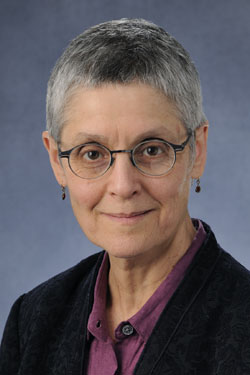
\includegraphics[width=\textwidth,valign=t]{roitman}

      \scriptsize Judith Roitman %(* 1945)
      \medskip

      \emph{Mainstream mathematics is beginning to see results using
      modern set theoretic techniques.}
    \end{column}
  \end{columns}
\end{frame}

{\usebackgroundtemplate{\begin{minipage}{\paperwidth}\vspace*{3.59cm}
\includegraphics[width=\paperwidth]{staircase}\end{minipage}}
\begin{frame}{The modal set-theoretic multiverse}
  \begin{tikzpicture}[remember picture,overlay]
    \node[xshift=-2.5cm,yshift=-4cm] at (current page.north east)
    {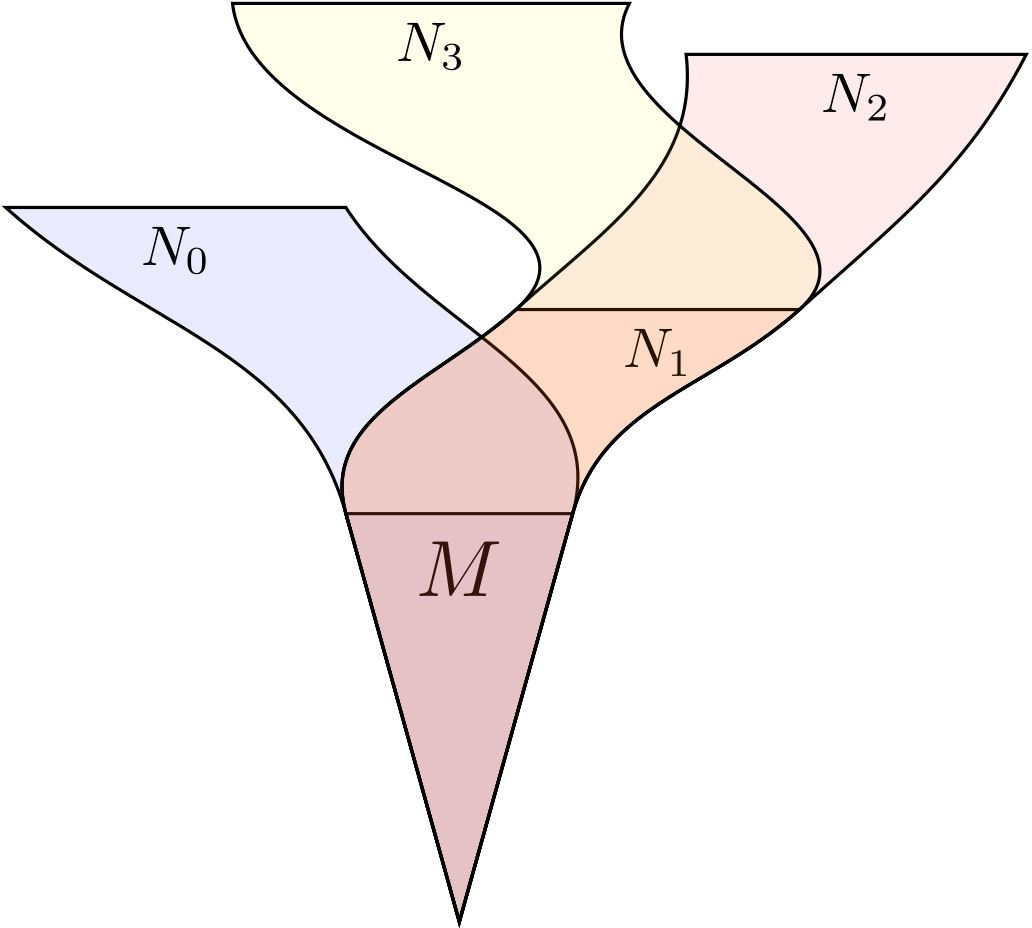
\includegraphics[width=3cm]{branching}};
  \end{tikzpicture}
  \justifying
  \vspace*{-2em}

  \textbf{Def.} A \hil{model of set theory} is a (perhaps class-sized) structure $(M,{\in})$
  satisfying axioms such as those of~\textsc{zfc}.

  {\small\emph{Examples.}\vspace*{-0.8em}
  \begin{itemize}
    \item $V$, the class of all sets \vspace*{-0.6em}
    \item $L$, Gödel's constructible universe \vspace*{-0.6em}
    \item $V[G]$, a forcing extension containing a generic filter~$G$ of \\ some
    poset of forcing conditions \vspace*{-0.6em}
    \item Henkin/term models from consistency of (extensions of)~\textsc{zfc}
  \end{itemize}}
  \pause

  \emph{We embrace all models of set theory:}

  \textbf{Def.} $\possible\varphi$ iff~$\varphi$ holds in \hil{some extension} of
  the current universe. \\
  \phantom{\textbf{Def.}} $\necessary\varphi$ iff~$\varphi$ holds in \hil{all extensions}
  of the current universe.
  \begin{itemize}
    \item $\necessary(\possible\textsc{CH} \wedge \possible\neg\text{CH})$,
    the continuum hypothesis is a \hil{switch}.
    \item $\necessary\possible\necessary(\text{$X$ is countable})$,
    existence of an enumeration is a \hil{button}.
  \end{itemize}
\end{frame}}

\begin{frame}{The modal topos-theoretic multiverse}
  \textbf{Def.} A statement~$\varphi$ holds \ldots
  \begin{enumerate}
    \small
    \item \hil{everywhere} ($\necessary\varphi$) iff it holds in every topos
    (over the current base).
    \item \hil{somewhere} ($\possible\varphi$) iff it holds in some positive topos.
    \item \hil{proximally} ($\xpossible\varphi$) iff it holds in some positive overt topos.
  \end{enumerate}
  \bigskip

  \begin{tikzpicture}[overlay]
    \node[anchor=south east,inner sep=0] (image) at (14.8,0.2) {
      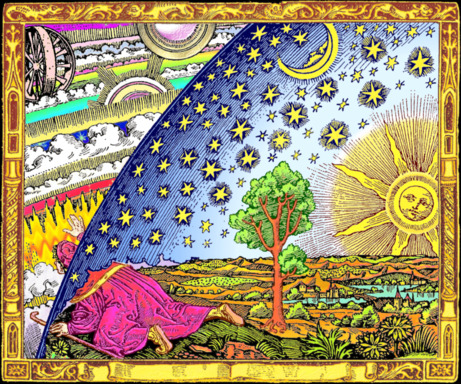
\includegraphics[width=0.2\textwidth]{multiverse}
    };
  \end{tikzpicture}\vspace*{-2.3em}

  \pause

  \small
  \begin{multicols}{2}
    For every inhabited set~$X$, \emph{proximally} \\
    there is an enumeration~$\NN \twoheadrightarrow X$.
    \medskip

    A quasiorder is well iff \emph{everywhere}, \\
    every sequence is good.
    \medskip

    A ring element is nilpotent iff \\
    all prime ideals \emph{everywhere} contain it.
    \medskip

    For every ring, \emph{proximally} \\ there is a maximal ideal.
    \medskip

    A relation is well-founded iff \emph{everywhere}, \\ there is no descending chain.
    \medskip

    \emph{Somewhere}, \\ the law of excluded middle holds.
  \end{multicols}
  \pause

  \begin{block}{}
    \justifying
    \textbf{Prop.} Let~$(X,{\leq})$ be a well quasiorder.
    Then~$({<})$, where~$x < y \equiv (x \leq y \wedge \neg(y \leq x))$,
    is well-founded.
  \end{block}
  \vspace*{-0.5em}

  \emph{Proof.} Everywhere, there can be no infinite descending chain, as any
  such would also be good. \qed

  Unrolling this proof gives a program~$\nabla\mathsf{Good}\,\varepsilon \to
  \prod_{x:X} \mathsf{Acc}\,x$.
\end{frame}

\begin{frame}{The modal type-theoretic multiverse?}
  \emph{As I understand it, \ldots}

  For extensional type theory, similar picture as with toposes:
  Given a model of extensional type theory and a Grothendieck site~$\mathcal{C}$ in it, there
  is a model of extensional type theory deserving the name~``sheaf model
  over~$\mathcal{C}$''. This sheaf model is just a thin translation layer of
  the base model.
  \pause

  For HoTT-like theories, given a ``presheaf model'' we know how to construct a
  ``sheaf model'', but we do not know how to construct presheaf models in the
  first place.
  \pause

  Still, can pragmatically use~$\nabla$ and feel philosophically inspired.
\end{frame}

\end{document}
